\documentclass[14pt,a4paper,final]{extreport}
\nonstopmode
\usepackage[T2A]{fontenc}
\usepackage[utf8]{inputenc}
\DeclareUnicodeCharacter{0306}{~}
\usepackage[russian]{babel}
\usepackage[a4paper, top=2cm, bottom=2cm, left=2cm, right=1cm,marginparsep=.5cm]{geometry}
\usepackage{fancyhdr}
\usepackage[export]{adjustbox}
\usepackage{marginnote}
\usepackage{tabularray}
\usepackage{longtable}
\usepackage{ltablex}

\usepackage{amsmath}
\usepackage{amssymb}

\usepackage{enumitem}
\setlist[itemize]{leftmargin=\parindent,nosep}
\setlist[enumerate]{leftmargin=\parindent,nosep}
\renewcommand\labelitemi{--}

\usepackage[none]{hyphenat}
\usepackage{setspace}
\onehalfspacing 
\usepackage{float}
\usepackage{xpatch}

\usepackage{tocloft, titlesec, titletoc}
\usepackage{indentfirst}
\titleformat{\chapter}[block]{\normalfont\bfseries\large}{\thechapter}{1ex}{\centering\MakeUppercase}
\titlespacing*{\chapter}{0pt}{-\baselineskip}{2\baselineskip}

\titleformat{\section}[block]{\normalfont}{\thesection}{1ex}{\normalfont}
\titlespacing{\section}{1.25cm}{\baselineskip}{\baselineskip}

\usepackage[hidelinks]{hyperref}

%Оформление подразделов
\titleformat{\subsection}[block]{\normalfont}{\thesubsection}{1ex}{\normalfont}
\titlespacing{\subsection}{1.25cm}{\baselineskip}{\baselineskip}

%Оформление под-подразделов
\titleformat{\subsubsection}[block]{\normalfont}{\thesubsection}{1ex}{\normalfont}
\titlespacing{\subsubsection}{1.25cm}{0pt}{\baselineskip}

\usepackage{titlesec}

% Настройка глубины нумерации заголовков
\setcounter{secnumdepth}{3}
\setcounter{tocdepth}{3}

% Настройка внешнего вида заголовков с помощью titlesec
\titleformat{\subsubsection}[hang]{\normalfont\normalsize}{\thesubsubsection}{0.5em}{}

%\titlespacing{\subsubsection}{35pt}{\parskip}{\parskip}

%\setcounter{tocdepth}{4}%
%\setcounter{secnumdepth}{4}% Number \subsubsection
\renewcommand{\cftdotsep}{2.75}
\renewcommand{\cftchapfont}{\normalfont}
\renewcommand{\cfttoctitlefont}{\hfill\normalfont\large\bfseries}
\renewcommand{\cftaftertoctitle}{\hfill}
\renewcommand{\cftchapleader}{\cftdotfill{\cftdotsep}} % for chapters
\renewcommand{\cftsecleader}{\cftdotfill{\cftdotsep}}  % for sections
\renewcommand{\cftsubsecleader}{\cftdotfill{\cftdotsep}} % for subsections
\renewcommand{\cftsubsubsecleader}{\cftdotfill{\cftdotsep}} % for subsubsections
\setlength{\cftbeforetoctitleskip}{-.6\baselineskip}
\setlength{\cftaftertoctitleskip}{-\baselineskip}
\setlength{\cftbeforechapskip}{\baselineskip}
\renewcommand{\cftchappagefont}{}

\renewcommand{\contentsname}{СОДЕРЖАНИЕ\vspace{\baselineskip}}% (ГОСТ Р 7.0.11-2011, 4)
\addto{\captionsrussian}{\renewcommand{\bibname}{СПИСОК ИСПОЛЬЗОВАННОЙ ЛИТЕРАТУРЫ\bigskip}}

\makeatletter
\renewcommand\@biblabel[1]{#1.\ }
\makeatother

\let\mtcontentsname\contentsname\addto\captionsrussian{\typeout{foo}\renewcommand{\contentsname}{\MakeUppercase\mtcontentsname}}

\makeatletter
\patchcmd{\chapter}{\if@openright\cleardoublepage\else\clearpage\fi}{\vspace{3\baselineskip}}{}{}
\makeatother

\newcommand*\rot[1]{\rotatebox{90}{#1}}
\newlength{\rs}
\setlength{\rs}{.5mm}

\makeatletter
\AddEnumerateCounter{\asbuk}{\russian@alph}{щ}
\makeatother

\fancypagestyle{firststyle}
{
    \fancyhf{} % sets both header and footer to nothing
    \renewcommand{\headrulewidth}{0pt}
    \fancyfoot[C]{
    
        {\vspace{-\baselineskip}\normalfont\textbf{Москва 2026}}
    } 
}

\begin{document}
\pagenumbering{gobble}
\raggedbottom

%для изменения

\newcommand{\fullname}{Нагороднюк Алиса Дмитриевна}
\newcommand{\shname}{Нагроднюк А. Д.}
\newcommand{\grp}{М3О-225БВ-24}
\newcommand{\variant}{9} %номер варианта (если многозначный - уберите 0 в \cipher)
\newcommand{\fieldA}{\( \vec a = z^3 \vec i + x^3 \vec j + y^3 \vec k \)}
\newcommand{\fieldB}{\( \vec b = (y^3z^4 + 2xy) \vec i + (3xy^2z^4 + x^2) \vec j + (4xy^3z^3 + 2z) \vec k \)}

\newcommand{\cipher}{643.02066606.0000\variant}
\newcommand{\cipherlri}{643.02066606.\\0000\variant}
\newcommand{\docstamp}{\cipher-01 34 01}
\newcommand{\doctitle}{Программа визуализации\\эквипотенциальных поверхностей\\и силовых линий}
\newcommand{\doctitleoneline}{Программа визуализации эквипотенциальных поверхностей и силовых линий}
\newcommand{\programtitle}{VectorField}
\newcommand{\docname}{Руководство оператора}
\input{lu.tex}
\pagebreak

\input{title.tex}
\pagebreak

\parindent=1.25cm
\sloppy

\pagenumbering{arabic}
\setcounter{page}{2}

\pagestyle{fancy}

\fancypagestyle{plain}

\fancyhf{} % clear all header and footer fields

\fancyhead[C]{\bfseries\thepage\\\docstamp}

\renewcommand{\headrulewidth}{0pt}
\pagebreak

\chapter*{Аннотация}
\addcontentsline{toc}{chapter}{Аннотация}

В данном программном документе приведено руководство оператора по применению и эксплуатации программы «VectorField», предназначенной для  расчета и отображения параметров эквипотенциальных поверхностей и силовых линей двух полей.

В данном программном документе, в разделе «Назначение программы» указаны сведения о назначении программы и информация, достаточная для понимания функций программы и её эксплуатации. 

В разделе «Условия выполнения программы» указаны условия, необходимые для выполнения программы (минимальный состав аппаратных и программных средств и т.п.).

В данном программном документе, в разделе «Выполнение программы» указана последовательность действий оператора, обеспечивающих загрузку, запуск, выполнение и завершение программы, приведено описание функций, формата и возможных вариантов команд, с помощью которых оператор осуществляет загрузку и управляет выполнением программы, а также ответы программы на эти команды.

В разделе «Сообщения оператору» приведены тексты сообщений, выдаваемых в ходе выполнения программы, описание их содержания и соответствующие действия оператора (действия оператора в случае сбоя, возможности повторного запуска программы и т.п.).

\pagebreak

\addcontentsline{toc}{chapter}{Содержание}

\tableofcontents
\pagebreak

\chapter{ НАЗНАЧЕНИЕ ПРОГРАММЫ}
\section{ Функциональное назначение программы}
Функциональным назначением программы является: 

\begin{enumerate}[label=\arabic*.]
	\item Выбрав следующие обозначения: \( S_{xy} \), \( S_{yz} \), \( S_{xz} \) --- части координатных плоскостей \( xOy \), \( yOz \), \( xOz \) соответственно, замыкающие поверхность \( S \) до замкнутой поверхности \( S_c \); \( S_c = S \bigcup S_{xy} \bigcup S_{yz} \bigcup S_{xz} \); \( A \), \( B \), \( C \) --- точки поверхности \( S \), лежащие на осях \( Ox \), \( Oy \), \( Oz \) соответственно; \( ABCD \) --- замкнутый контур поверхности \( S \), по которому вычисляется циркуляция,  определить класс поля \( \vec a \), вычислив  \( \mathrm{div} \, \vec a \),  \( \mathrm{rot} \, \vec a \):  \( \mathrm{div} \, \vec a = \frac{\partial a_x}{\partial x} + \frac{\partial a_y}{\partial y} + \frac{\partial a_z}{\partial z} \),
	\( \mathrm{rot} \, \vec a = \left| \begin{matrix}
		\vec i & \vec j & \vec k \\
		\frac{\partial}{\partial x} & \frac{\partial}{\partial y} & \frac{\partial}{\partial z} \\
		a_x & a_y & a_z \\
	\end{matrix} \right|
	= (\frac{\partial a_z}{\partial y} - \frac{\partial a_y}{\partial z})\vec i + (\frac{\partial a_x}{\partial z} - \frac{\partial a_z}{\partial x})\vec j + (\frac{\partial a_y}{\partial x} - \frac{\partial a_x}{\partial y})\vec k \);
	\item Вычислить поток \( P \) поля \( \vec a \) через поверхность \( S \) в направлении внешней нормали для сферы:
	\begin{enumerate}[label=\theenumi\arabic*]
		\item По формуле Гаусса-Остроградского: замыкаем поверхность \( S \)  поверхностями \( S_{xy} \), \( S_{yz} \), \( S_{xz} \) до замкнутой поверхности \( S_c \).
		Пусть  \( T \) - тело, ограниченное поверхностью  \( S_c \), а  \( P_c \) - поток поля \( \vec a \) через \( S_c \) в направлении внешней нормали.
		\( P_c = \iiint\limits_T \mathrm{div} \, \vec a\,dv \). 
		\bigskip
		\\Перейти к сферическим координатам по формулам \( x = \rho\cos\psi\cos\phi \); \( y = \rho\cos\psi\sin\phi \); \( z = \rho\sin\psi \); \( J = \rho^2\cos\psi \). 
		\bigskip
		\\Тогда \( P_c = 3\int_0^{\pi/2}{d\phi} \int_0^{\pi/2}{d\psi} \int_0^1{\rho\cos\psi\cos\phi\rho^2\cos\psi\,d\rho } = 3 \int_0^{\pi/2}\cos\phi d \phi \int_0^{\pi/2}\cos^2\psi d \psi \int_0^1\rho^3 d \rho \). \( P = P_c - P_{xy} - P_{yz} - P_{xz} \), где \( P_{xy}, P_{yz}, P_{xz} \) - потоки поля \( \vec a \) через поверхности \( S_{xy} \), \( S_{yz} \), \( S_{xz} \) соответственно;
		
		\item Вычислить поток непосредственно через поверхностный интеграл\\ \( P = \iint\limits_S xzdydz + xydzdx + yzdxdy \).
	\end{enumerate}
	
	\item Вычислить циркуляцию поля \( \vec a \) по замкнутому контуру \( ABCA \):

\pagebreak % разрыв страницы
	
	\begin{enumerate}[label=\theenumi\arabic*]
		\item по формуле Стокса \( C = \iint\limits_S \mathrm{rot}_n \, \vec a dS \);
		
		\item непосредственно с помощью криволинейного интеграла \( C = \oint\limits_{(ABCD)_+}{a_xdx + a_ydy + a_zdz} \).
	\end{enumerate}
	
	\item Изучить поле \( \vec b \):
	
	\begin{enumerate}[label=\theenumi\arabic*]
		\item Проверить потенциальность поля \( \vec b \). Убедиться, что ротор поля равен нулю: \( \mathrm{rot} \, \vec b = (\frac{\partial b_z}{\partial y} - \frac{\partial b_y}{\partial z})\vec i + (\frac{\partial b_x}{\partial z} - \frac{\partial b_z}{\partial x})\vec j + (\frac{\partial b_y}{\partial x} - \frac{\partial b_x}{\partial y})\vec k = 0 \);
		
		\item Вычислить потенциал \( \varphi \) поля \( b \) по формуле \( \varphi = \int_0^x{b_x(x,0,0)\,dx} + \int_0^y{b_y(x,y,0)\,dy} +\int_0^z{b_z(x,y,z)\,dz} \);
		
		\item Проверить истинность найденного потенциала: \\\( \varphi'_x = b_x\mathrm{,}\;\varphi'_y = b_y\mathrm{,}\;\varphi'_z = b_z \);
		
		\item Вычислить с помощью потенциала \( \varphi \) работу \( W \) сил поля по перемещению материальной точки из точки \(O(0,0,0) \) в точку \( M(1,1,1) \) по формуле $W = \varphi(1, 1, 1,) - \varphi(0, 0, 0)$.
	\end{enumerate}

\addtocounter{page}{0}
\fancyhead[C]{\bfseries\thepage\\\docstamp}  % верхний колонтитул
	
	\item Построить силовые линии для векторного поля в базисе \( \vec i \), \( \vec j \), \( \vec k \) для поля \( \vec a \) или \( \vec b \):
	
	\begin{enumerate}[label=\theenumi\arabic*]
		\item решить систему уравнений \[ \frac{dx}{a_x(x, y, z)} = \frac{dy}{a_y(x, y, z)} = \frac{dz}{a_z(x, y, z)} \]  и получить два семейства \( F_1(x, y, z) = C_1 \), \( F_2(x, y, z) = C_2 \) пространственных поверхностей;
		
		\item построить силовые линии по линиям пересечения этих семейств \( F_1(x, y, z)~=~C_1 \) и \( F_2(x, y, z)~=~C_2 \) пространственных поверхностей.
	\end{enumerate}
	
	\item Построить эквипотенциальные поверхности для векторного поля в базисе \( \vec i \), \( \vec j \), \( \vec k \) для поля \( \vec a \) или \( \vec b \):
	
	\begin{enumerate}[label=\theenumi\arabic*]
		\item определить потенциал \( \varphi \) с использованием связи между полем и потенциалом: \[ \vec a = -\nabla \varphi ;\]
		
		\item решить уравнение Лапласа \[ \nabla^2 \varphi = 0, \]найдя функцию потенциала \( \varphi (x, y, z) \) из уравнения Лапласа;
\pagebreak % разрыв страницы
		
		\item построить эквипотенциальные поверхности, решив уравнение \[ \varphi (x, y, z) = \mathrm{const} .\]
	\end{enumerate}
\end{enumerate}

\section{ Эксплуатационное назначение программы}
Программа создается с целью расчета и моделирования элементов теории поля.

\section{ Состав функций, процедур и методов}
\begin{itemize}
	\item  wWinMain
	\item  MyRegisterClass
	\item  InitInstance
	\item  ShowOpenFileDialog
	\item  ShowSaveFileDialog
	\item  ReadFromFile
	\item  SaveToFile
	\item  ShowErro
	\item  WndProc
	\item  HandlePaint
	\item  DrawVisualization
	\item  GetDrawCoords
	\item  DrawLabels
	\item  GenerateWolframPlot
	\item  WriteScript
	\item  RunWolfram
	\item  CalculationsClassRegister
	\item  CalculationsWndProc
	\item  FieldClassRegister
	\item  FieldWndProc
	\item  InputClassRegister
	\item  InputWndProc
	\item  KeyboardInputClassRegister
	\item  KeyboardInputWndProc
	\item  PartialDerivative
	\item  TrippleIntegralInSphericalCordinates
	\item  DoubleIntegralInPolarCoordinates
	\item  Integral
	\item  PowerLinesClassRegister
	\item  PowerLinesWndProc
	\item  SettingsClassRegister
	\item  SettingsWndProc
	\item  Divergence
	\item  Rotor
	\item  CheckClass
	\item  GaussOstrogradskyFormulaForOktantOfBall
	\item  SurfaceIntegralOverTheSurfaceOfOktant
	\item  StocksFormula
	\item  CirculationOverLineIntegral
	\item  Potential
	\item  Polynomial::Polynomial
	\item  Polynomial::Add
	\item  Polynomial::Evaluate
	\item  Polynomial::SetVariableToZero
	\item  Polynomial::IntegrateSymbolically
	\item  Polynomial::ToWString
	\item  PolyToWolframString
\end{itemize}

\subsection{Функция wWinMain}
Определяет точку входа в приложение. Осуществляется без вмешательства пользователя. 
В случае возникновения ошибки, пользователь получит соответствующее уведомление.

\subsection{Функция MyRegisterClass}
Регистрирует класс главного окна. Осуществляется без вмешательства пользователя. 
В случае возникновения ошибки, пользователь получит соответствующее уведомление.

\subsection{Функция InitInstance}
Сохраняет маркер экземпляра и создает главное окно. Осуществляется без вмешательства пользователя. 
В случае возникновения ошибки, пользователь получит соответствующее уведомление.

\subsection{Процедура ShowOpenFileDialog}
Отображает окно открытия файла. Осуществляется без вмешательства пользователя. 
В случае возникновения ошибки, пользователь получит соответствующее уведомление.

\subsection{Процедура ShowSaveFileDialog}
Отображает окно сохранения файла. Осуществляется без вмешательства пользователя. 
В случае возникновения ошибки, пользователь получит соответствующее уведомление.

\subsection{Процедура ReadFromFile}
Производит чтение из файла. Осуществляется без вмешательства пользователя. 
В случае возникновения ошибки, пользователь получит соответствующее уведомление.

\subsection{Процедура SaveToFile}
Производит запись в файл.  Осуществляется без вмешательства пользователя. 
В случае возникновения ошибки, пользователь получит соответствующее уведомление.

\subsection{Функция WndProc}
Обрабатывает сообщения в главном окне. Осуществляется без вмешательства пользователя. 
В случае возникновения ошибки, пользователь получит соответствующее уведомление.

\subsection{Процедура HandlePaint}
Выполняет отрисовку содержимого главного окна при обработке сообщения WM\_PAINT. Осуществляется без вмешательства пользователя. 
В случае возникновения ошибки, пользователь получит соответствующее уведомление.

\subsection{Функция CalculationsClassRegister}
Регистрирует класс окна расчётов. Осуществляется без вмешательства пользователя. 
В случае возникновения ошибки, пользователь получит соответствующее уведомление.

\subsection{Функция CalculationsWndProc}
Функция обработки сообщений в окне вывода рассчитанных параметров поля. Осуществляется без вмешательства пользователя. 
В случае возникновения ошибки, пользователь получит соответствующее уведомление.

\subsection{Функция FieldClassRegister}
Регистрирует класс окна визуализации. Осуществляется без вмешательства пользователя. 
В случае возникновения ошибки, пользователь получит соответствующее уведомление.

\subsection{Функция FieldWndProc}
Функция обработки сообщений в окне вывода визуализации поля. Осуществляется без вмешательства пользователя. 
В случае возникновения ошибки, пользователь получит соответствующее уведомление.

\subsection{Функция InputClassRegister}
Регистрирует класс окна ввода. Осуществляется без вмешательства пользователя. 
В случае возникновения ошибки, пользователь получит соответствующее уведомление.

\subsection{Функция InputWndProc}
Функция обработки сообщений в окне ввода. Осуществляется без вмешательства пользователя. 
В случае возникновения ошибки, пользователь получит соответствующее уведомление.

\subsection{Функция KeyboardInputClassRegister}
Регистрирует класс окна ввода с клавиатуры. Осуществляется без вмешательства пользователя. 
В случае возникновения ошибки, пользователь получит соответствующее уведомление.

\subsection{Функция KeyboardInputWndProc}
Функция обработки сообщений в окне ввода с клавиатуры. Осуществляется без вмешательства пользователя. 
В случае возникновения ошибки, пользователь получит соответствующее уведомление.

\subsection{Функция PartialDerivative}
Расчитывает и возвращает значение частной производной по переменной в точке. Осуществляется без вмешательства пользователя. 
В случае возникновения ошибки, пользователь получит соответствующее уведомление.

\subsection{Функция TrippleIntegralInSphericalCordinates}
Расчитывает и возвращает значение тройного интеграла в сферических координатах. Осуществляется без вмешательства пользователя. 
В случае возникновения ошибки, пользователь получит соответствующее уведомление.

\subsection{Функция DoubleIntegralInPolarCoordinates}
Расчитывает и возвращает значение двойного интеграла в полярных координатах. Осуществляется без вмешательства пользователя. 
В случае возникновения ошибки, пользователь получит соответствующее уведомление.

\subsection{Функция Integral}
Расчитывает и возвращает значение интеграла Римана. Осуществляется без вмешательства пользователя. 
В случае возникновения ошибки, пользователь получит соответствующее уведомление.

\subsection{Функция PowerLinesClassRegister}
Регистрирует класс окна визуализации силовых линий. Осуществляется без вмешательства пользователя. 
В случае возникновения ошибки, пользователь получит соответствующее уведомление.

\subsection{Функция PowerLinesWndProc}
Функция обработки сообщений в окне визуализации силовых линий. Осуществляется без вмешательства пользователя. 
В случае возникновения ошибки, пользователь получит соответствующее уведомление.

\subsection{Функция SettingsClassRegister}
Регистрирует класс окна настроек. Осуществляется без вмешательства пользователя. 
В случае возникновения ошибки, пользователь получит соответствующее уведомление.

\subsection{Функция SettingsWndProc}
Функция обработки сообщений в окне настроек. Осуществляется без вмешательства пользователя. 
В случае возникновения ошибки, пользователь получит соответствующее уведомление.

\subsection{Функция Divergence}
Расчитывает дивергенцию в точке. Осуществляется без вмешательства пользователя. 
В случае возникновения ошибки, пользователь получит соответствующее уведомление.

\subsection{Функция Rotor}
Расчитывает ротор в точке. Осуществляется без вмешательства пользователя. 
В случае возникновения ошибки, пользователь получит соответствующее уведомление.

\subsection{Функция CheckClass}
Определяет тип поля. Осуществляется без вмешательства пользователя. 
В случае возникновения ошибки, пользователь получит соответствующее уведомление.

\subsection{Функция GaussOstrogradskyFormulaForOktantOfBall}
Вычисляет поток по формуле Гаусса-Остроградского для октанта шара. Осуществляется без вмешательства пользователя. 
В случае возникновения ошибки, пользователь получит соответствующее уведомление.

\subsection{Функция SurfaceIntegralOverTheSurfaceOfOktant}
Вычисляет поток через поверхность шара, используя двойной интеграл в полярных координатах. Осуществляется без вмешательства пользователя. 
В случае возникновения ошибки, пользователь получит соответствующее уведомление.

\subsection{Функция StocksFormula}
Осуществляет расчёт по формуле Стокса. Осуществляется без вмешательства пользователя. 
В случае возникновения ошибки, пользователь получит соответствующее уведомление.

\subsection{Функция CirculationOverLineIntegral}
Вычисляет циркуляцию при помощи криволинейного интеграла. Осуществляется без вмешательства пользователя. 
В случае возникновения ошибки, пользователь получит соответствующее уведомление.

\subsection{Функция Potential}
Вычисляет потенциал поля в точке. Осуществляется без вмешательства пользователя. 
В случае возникновения ошибки, пользователь получит соответствующее уведомление.

\subsection{Метод Polynomial::Polynomial}
Конструктор класса многочлена, выполняющий инициализацию внутренних структур данных. Осуществляется без вмешательства пользователя. 
В случае возникновения ошибки, пользователь получит соответствующее уведомление.

\subsection{Метод Polynomial::Add}
Выполняет сложение текущего многочлена с другим многочленом с последующим приведением подобных слагаемых. Осуществляется без вмешательства пользователя. 
В случае возникновения ошибки, пользователь получит соответствующее уведомление.

\subsection{Метод Polynomial::Evaluate}
Производит численное вычисление значения многочлена в точке (x, y, z). Осуществляется без вмешательства пользователя. 
В случае возникновения ошибки, пользователь получит соответствующее уведомление.

\subsection{Процедура ShowError}
Отображает диалоговое окно с сообщением об ошибке в зависимости от переданного кода. Осуществляется без вмешательства пользователя. 
В случае возникновения ошибки, пользователь получит соответствующее уведомление.

\subsection{Процедура DrawVisualization}
Отрисовывает сгенерированное растровое изображение визуализации векторного поля на заданном контексте устройства. Осуществляется без вмешательства пользователя. 
В случае возникновения ошибки, пользователь получит соответствующее уведомление.

\subsection{Процедура GetDrawCoords}
Вычисляет координаты размещения изображения визуализации для корректного отображения в окне программы Осуществляется без вмешательства пользователя. 
В случае возникновения ошибки, пользователь получит соответствующее уведомление.

\subsection{Процедура DrawLabels}
Выводит текстовые подписи и пояснительные элементы для графиков визуализации. Осуществляется без вмешательства пользователя. 
В случае возникновения ошибки, пользователь получит соответствующее уведомление.

\subsection{Функция GenerateWolframPlot}
Координирует процесс построения визуализации, вызывая формирование скрипта, его выполнение и загрузку результирующего изображения в память. Осуществляется без вмешательства пользователя. 
В случае возникновения ошибки, пользователь получит соответствующее уведомление.

\subsection{Функция WriteScriptt}
Формирует файл скрипта на языке Wolfram Language, содержащий инструкции для построения графиков и экспорта их в растровый формат. Осуществляется без вмешательства пользователя. 
В случае возникновения ошибки, пользователь получит соответствующее уведомление.

\subsection{Функция RunWolfram}
Осуществляет вызов внешнего интерпретатора WolframScript для выполнения сгенерированного файла скрипта. Осуществляется без вмешательства пользователя. 
В случае возникновения ошибки, пользователь получит соответствующее уведомление.

\subsection{Метод Polynomial::SetVariableToZero}
Возвращает новый многочлен, в котором указанные переменные приравнены к нулю, отсеивая соответствующие слагаемые. Осуществляется без вмешательства пользователя. 
В случае возникновения ошибки, пользователь получит соответствующее уведомление.

\subsection{Метод Polynomial::IntegrateSymbolically}
Выполняет символьное (аналитическое) интегрирование многочлена по заданной переменной. Осуществляется без вмешательства пользователя. 
В случае возникновения ошибки, пользователь получит соответствующее уведомление.

\subsection{Метод Polynomial::ToWString}
Преобразует многочлен в удобное для чтения строковое представление. Осуществляется без вмешательства пользователя. 
В случае возникновения ошибки, пользователь получит соответствующее уведомление.

\subsection{Функция PolyToWolframString}
Преобразует многочлен в строковый формат, совместимый с синтаксисом WolframScript для последующей визуализации. Осуществляется без вмешательства пользователя. 
В случае возникновения ошибки, пользователь получит соответствующее уведомление.

\chapter{УСЛОВИЯ ВЫПОЛНЕНИЯ ПРОГРАММЫ}

\section{Минимальный состав аппаратных средств}

В состав технических средств должен входить \texttt{IBM}-совместимый персональный компьютер
(ПЭВМ), включающий в себя:
\begin{enumerate}[label=\asbuk*),ref=\asbuk*]
	\item Процессор \texttt{Intel Core i5} 2-ого поколения;
	\item Оперативную память объемом 256 Мб;
	\item Графический процессор \texttt{Intel HD Graphics 3000};
	\item Свободного места для хранения 64 Мб;
	\item Периферийные устройства такие как клавиатура, монитор с разрешением 1280 точек в ширину на 720 точек в высоту.
\end{enumerate}

\section{Минимальный состав программных средств}
Для обеспечения функционирования программы на компьютере, на котором будет эксплуатироваться данный программный продукт, должно быть установлено следующее программное обеспечение:

Наименование программы: C++,

Обозначение программы: C++,

Версия программного изделия: 15.0;

Наименование программы: Wolfram Engine,

Обозначение программы: Wolfram Engine,

Версия программного изделия: 15.0.



\section{Требования к персоналу (пользователю)}

Минимальное количество персонала, требуемого для работы программы, должно включать в себя конечного пользователя программы -- оператора.

Пользователь должен быть ознакомлен с инструкцией пользователя.

Конечный пользователь программы (оператор) должен обладать практическими навыками работы с графическим пользовательским интерфейсом операционной системы.



\chapter{ ВЫПОЛНЕНИЕ ПРОГРАММЫ}
\section{ Загрузка и запуск программы}

Для установки программного обеспечения необходимо иметь установленную интегрированную среду разработки Microsoft Visual Studio версии 2022 или выше с пакетом русского языка, а также Wolfram Engine версии 15.0 и выше.

Необходимо скачать архив «VectorField» и распаковать его.

Открыть распакованную папку «VectorField» и найти файл \texttt{VectorField.sln}. Нажать на найденный файл правой кнопкой мыши и выбрать «Открыть с помощью» -> «Microsoft Visual Studio 2022»  (рис. 3.1).

\begin{figure}[H]	
	
\includegraphics[width=0.95\linewidth]{pics/1.png}
	\label{fig:1}
	\caption{Загрузка программы}
\end{figure} 

После загрузки Microsoft Visual Studio и открытия основного окна среды разработки, необходимо нажать на кнопку <<Локальный отладчик Windows>>, расположенные наверху окна (рис. 3.2). После нажатия этой кнопки произойдет сборка проекта и открытие исполняемого файла программы.

\begin{figure}[H]	
	
\includegraphics[width=0.95\linewidth]{pics/2.png}
	\label{fig:2}
	\caption{Запуск программы}
\end{figure} 

\section{ Выполнение программы}

По завершении запуска программы откроется главная форма, на которой имеются следующие кнопки:

\begin{itemize}
	\item 1. Импорт данных;
	\item 2. Показать данные;
	\item 3. Расчёт данных;
	\item 4. Визуализация поля А;
	\item 5. Визуализация поля Б;
	\item 6. Экспорт в TXT.
\end{itemize}

По завершении загрузки программы откроется главная форма, на которой пользователю будет предложено загрузить входные данные из файла.

Главная кнопочная форма, изображённая на рис. 3.3, отображается при запуске программы и служит для открытия окон и выполнения действий по нажатию кнопок.
\begin{figure}[H]	
	
\includegraphics[width=0.95\textwidth]{pics/3.png}
	\label{fig:gkf}
	\caption{Главная кнопочная форма}
\end{figure}

\subsection{Импорт данных}
По нажатии кнопки происходит открытие окна проводника Windows с возможностью загрузки файла с параметрами поля, изображённое на рис. 3.4. Оператор может загрузить файл, содержащий корректные данные.
\begin{figure}[H]	
	
\includegraphics[width=0.95\textwidth]{pics/4.png}
	\caption{Импорт данных}
	\label{fig:kip}
\end{figure}

\subsection{Показать данные}
По нажатии кнопки происходит расчёт параметров поля. Результат выводится в форме на рис. 3.5.
\begin{figure}[H]	
	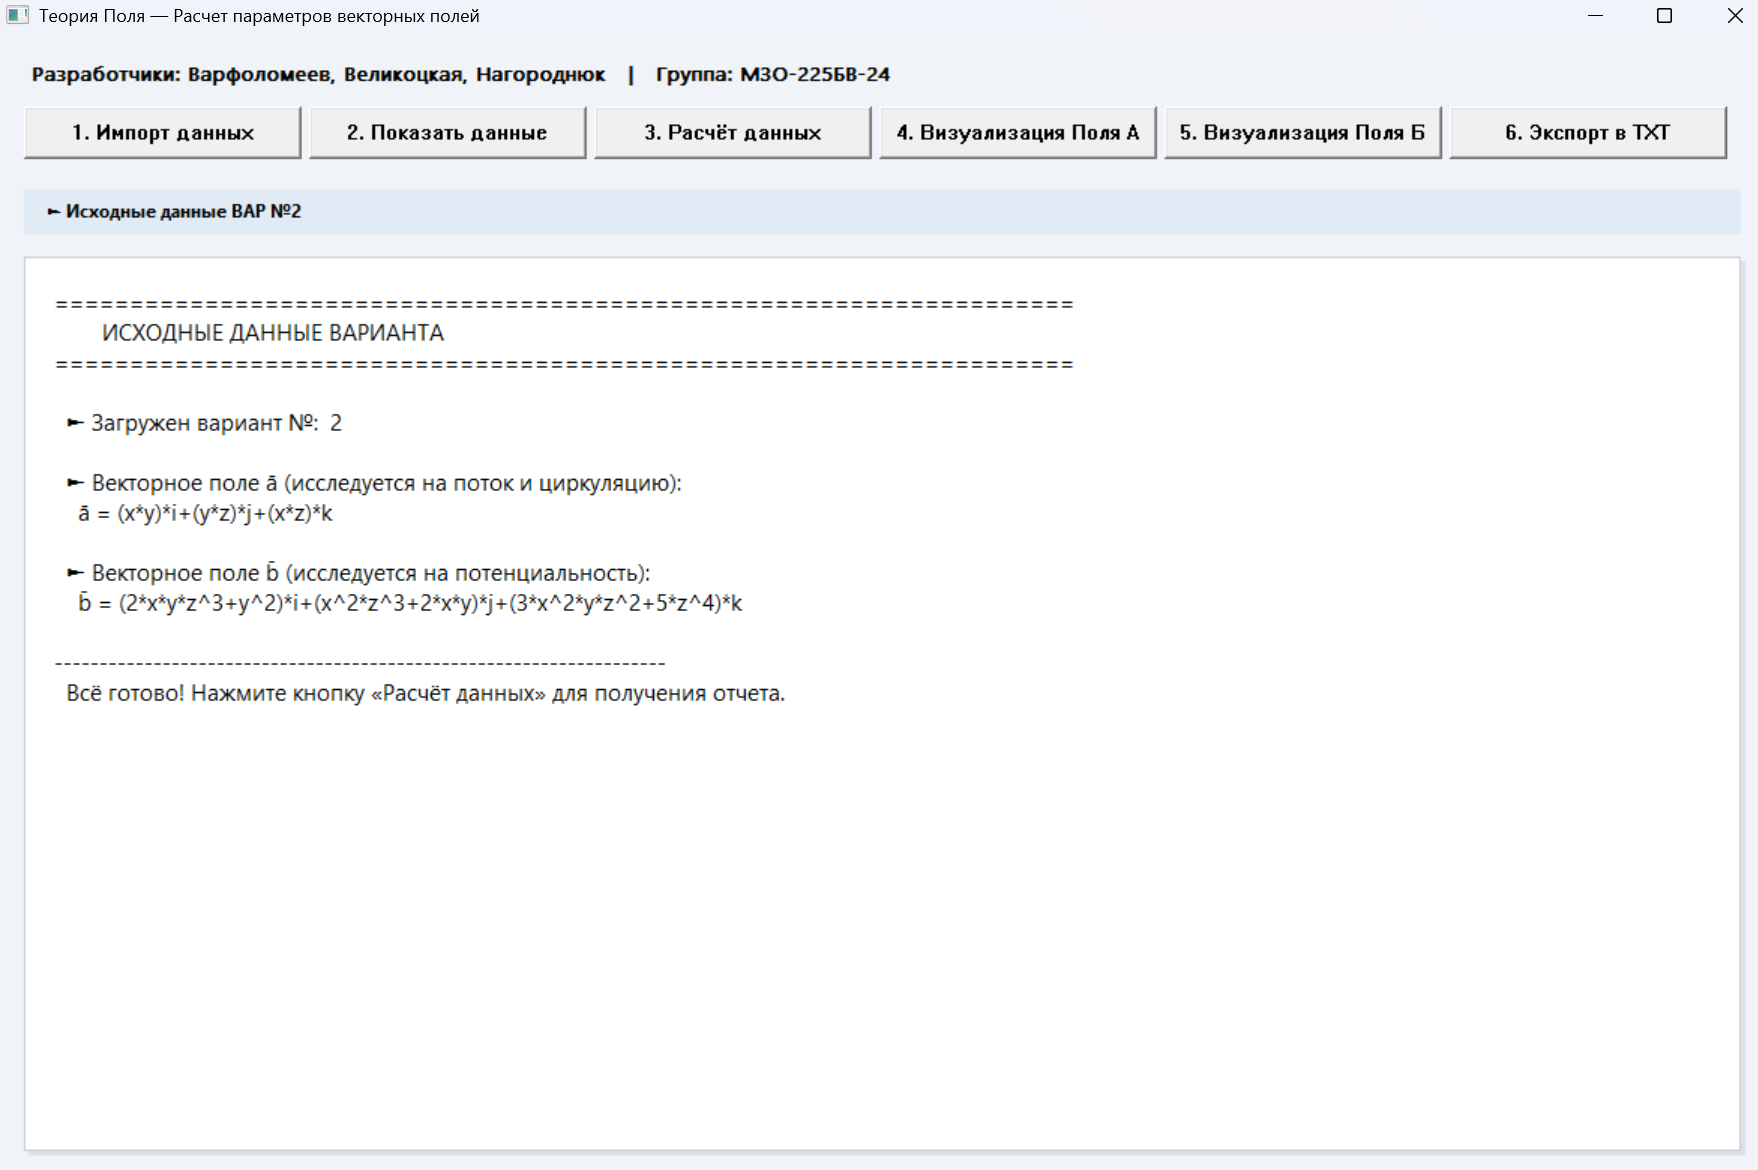
\includegraphics[width=0.95\textwidth]{pics/5.png}
	\caption{Показать данные}
	\label{fig:show}
\end{figure}

\subsection{Расчет данных}
По нажатии кнопки происходит расчёт параметров поля. Результат выводится в форме на рис. 3.6.
\begin{figure}[H]	
	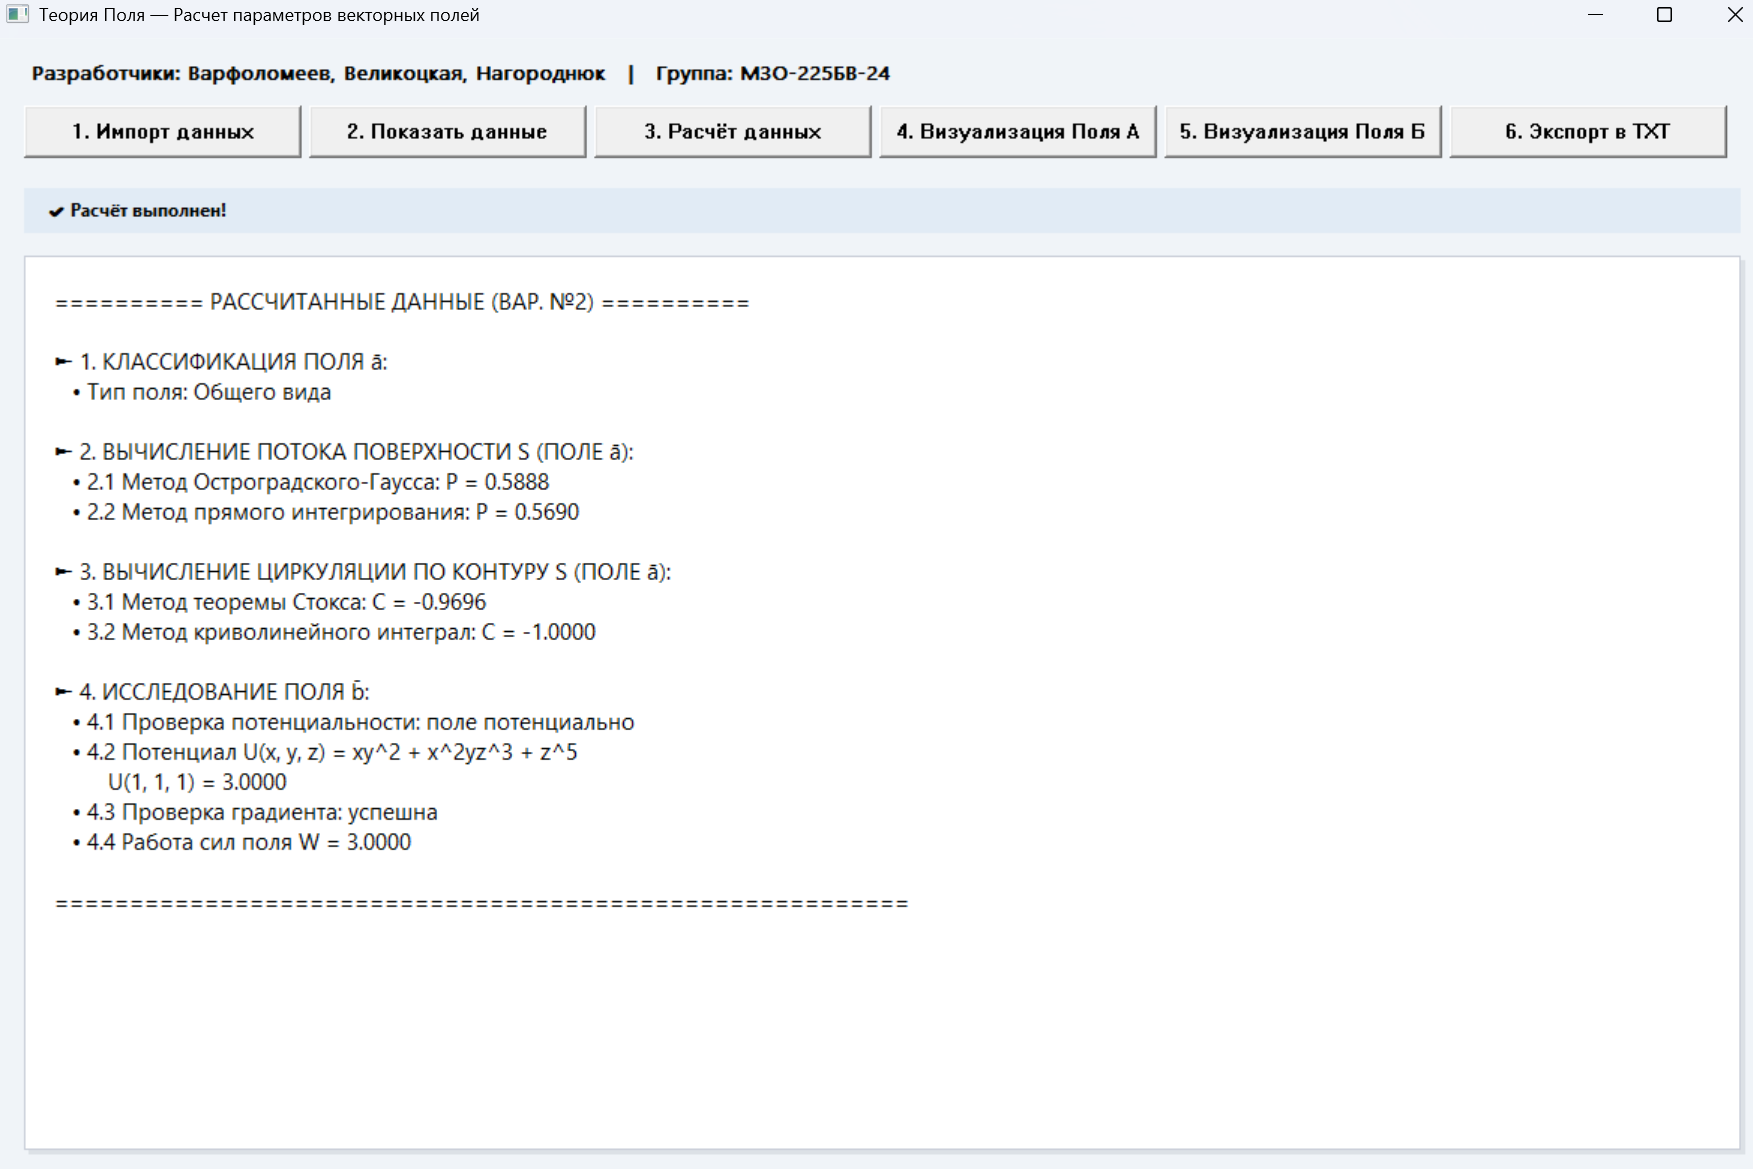
\includegraphics[width=0.95\textwidth]{pics/6.png}
	\caption{Расчет данных}
	\label{fig:calcfield}
\end{figure}

\subsection{Визуализация Поля А}
По нажатии кнопки происходит визуализация силовых линий поля a. Результат выводится в форме на рис. 3.7.
\begin{figure}[H]	
	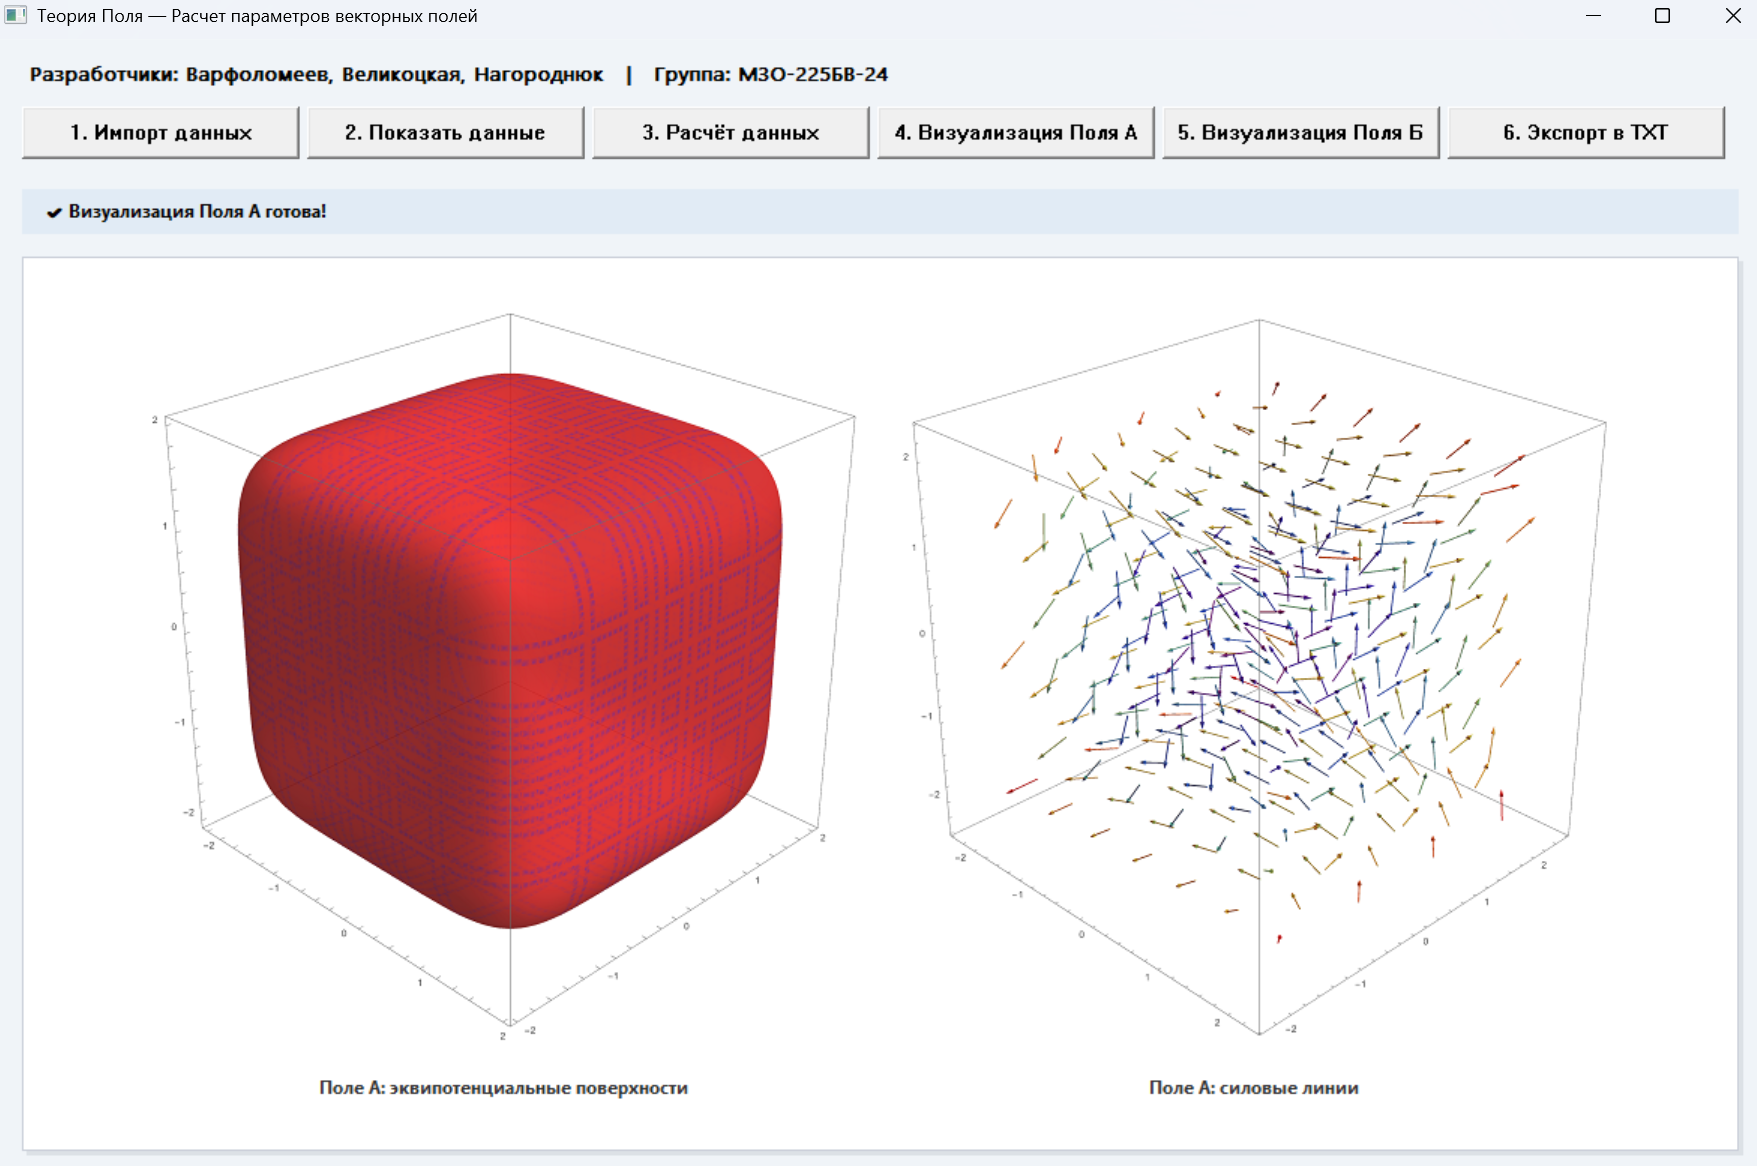
\includegraphics[width=0.95\textwidth]{pics/7.png}
	\caption{Визуализация Поля А}
	\label{fig:linesa}
\end{figure}

\subsection{Визуализация Поля Б}
По нажатии кнопки происходит визуализация силовых линий поля b. Результат выводится в форме на рис. 3.8.
\begin{figure}[H]	
	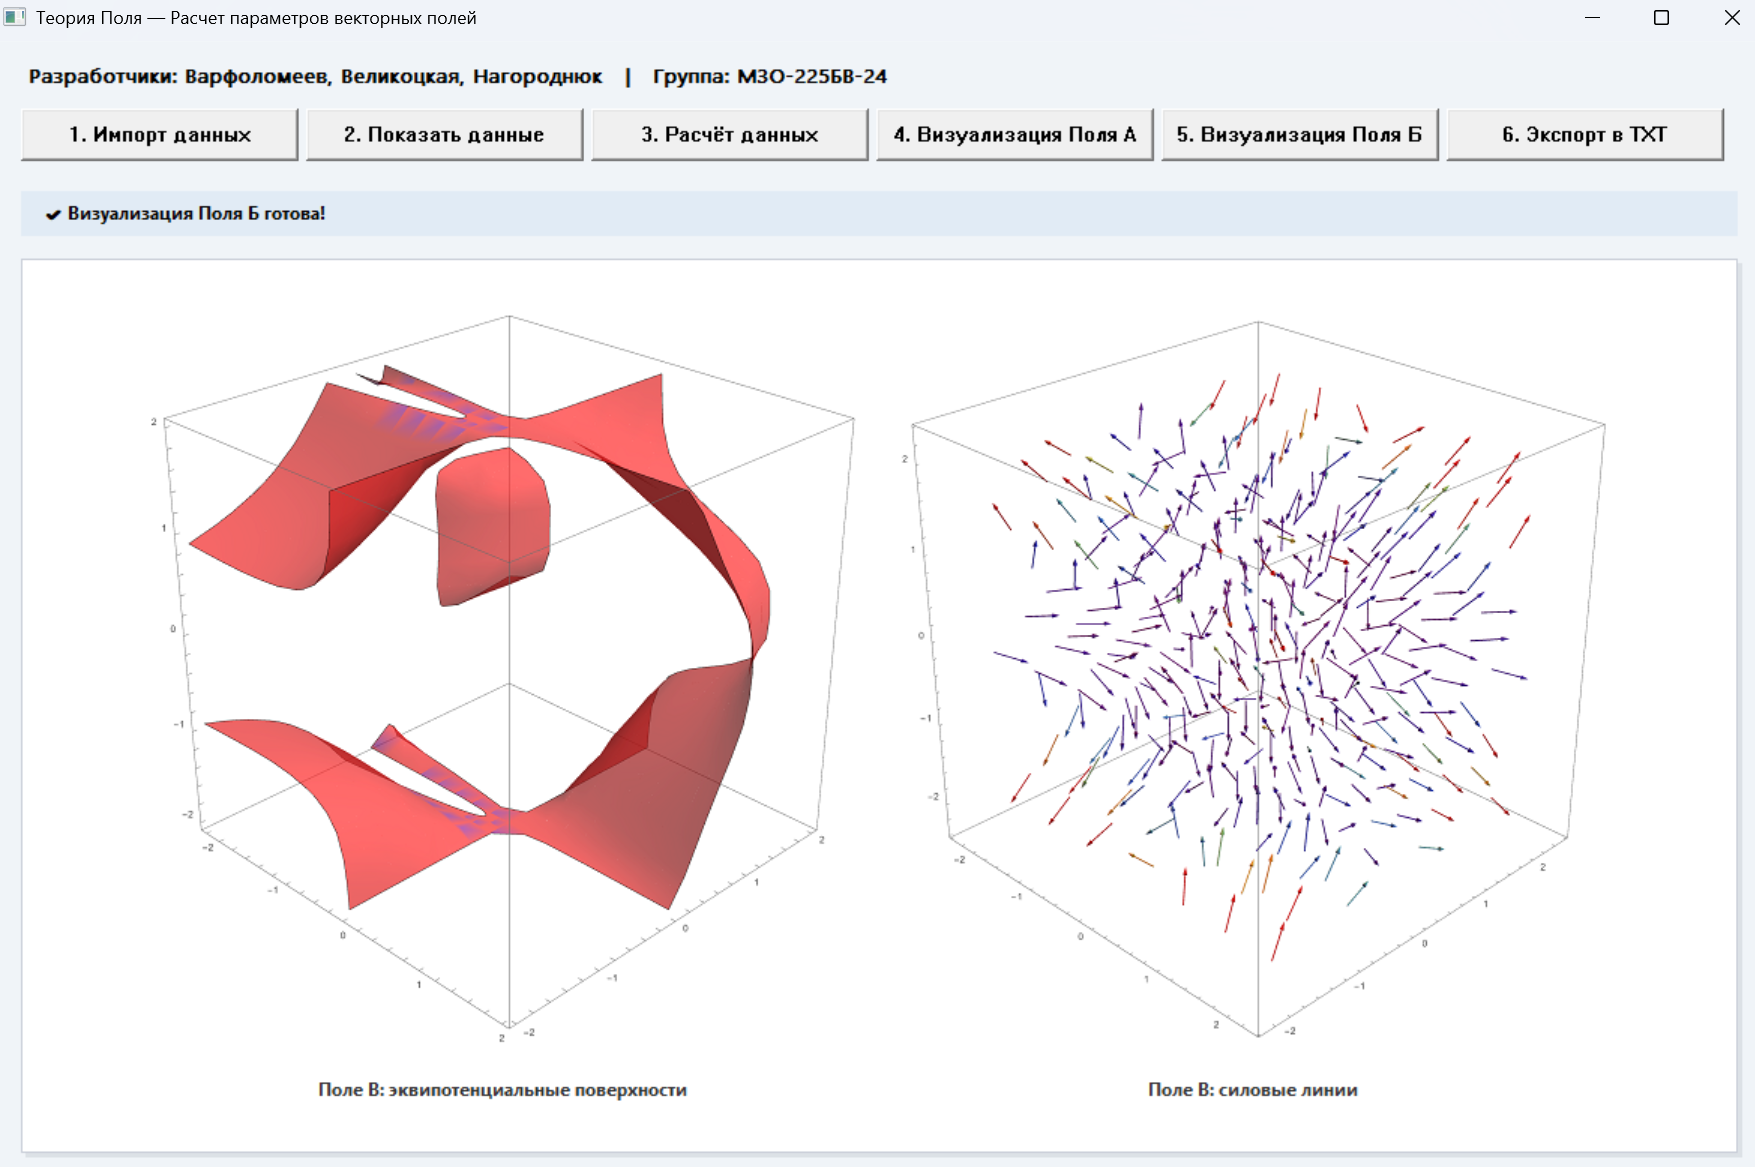
\includegraphics[width=0.95\textwidth]{pics/8.png}
	\caption{Визуализация Поля Б}
	\label{fig:linesb}
\end{figure}

\subsection{Экспорт в TXT}
По нажатии кнопки происходит открытие окна проводника  Windows с возможностью экспорта файла с результатами расчетов, изображённое на рис. 3.9. Оператор может сохранить файл при помощи этого окна.
\begin{figure}[H]	
	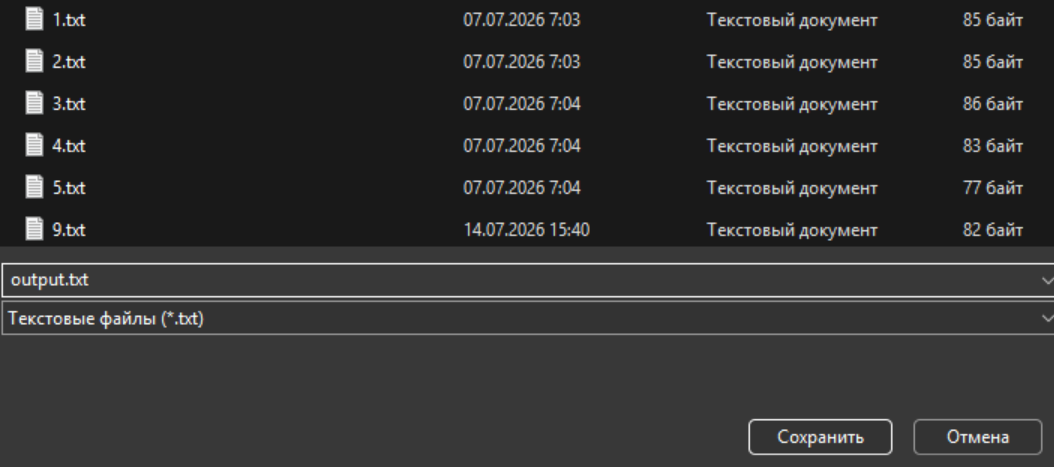
\includegraphics[width=0.95\textwidth]{pics/9.png}
	\caption{Экспорт в TXT}
	\label{fig:export}
\end{figure}

\section{ Завершение работы программы}
Завершение работы программы осуществляется путем закрытия главной кнопочной формы средствами Windows или Visual Studio.


\chapter{СООБЩЕНИЯ ОПЕРАТОРУ}
\section{Специальные сообщения оператору во время работы программы}
Выдаётся пользователю в случае возникновения ошибок во время выполнения программы. 

Сообщение содержит в себе информацию о причине возникновения ошибки и месте ее возникновения. Пример сообщения приведён на рис. 4.1.

\begin{figure}[H]	
	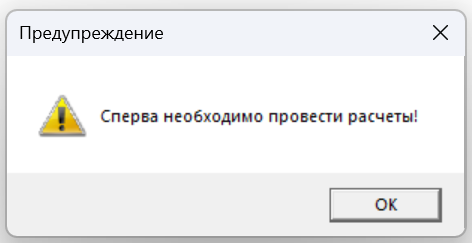
\includegraphics[width=0.95\linewidth]{pics/10.png}
	\label{fig:6}
	\caption{Пример сообщения об ошибке}
\end{figure} 

\pagebreak

\label{lastpage}

%\newcounter{totalpages}
%\setcounter{totalpages}{\pageref{lastpage}}
%\addtocounter{totalpages}{5}


\addcontentsline{toc}{chapter}{Лист регистрации изменений}
\renewcommand{\headrulewidth}{0pt}
\fontsize{3.5mm}{3mm}\selectfont
\noindent\begin{tblr}{colspec={|[\rs]p{8mm,c}|X[20,c]|X[20,c]|X[20,c]|X[20,c]|X[20,c]|X[25,c]|X[25,c]|X[15,c]|X[12,c]|[2pt]},
             rows   = {5mm},
             row{1} = {10mm,m},
             row{2} = {5mm,m},
             row{3} = {20mm,m},
             rowsep = 0pt,colsep = 0pt,
             vline{2-10} = {2-3}{\rs}
}\hline[\rs]
\SetCell[c=10]{c} {\fontsize{7mm}{0mm}\selectfont Лист регистрации изменений} &&&&&&&&&&& \\\hline[\rs]
\SetCell[c=5]{c} {\small Номера листов (страниц)} &&&&& \SetCell[r=2]{c} Всего листов (страниц) в документе & \SetCell[r=2]{c} № документа & \SetCell[r=2]{c} {Входящий № сопроводи-\\тельного  документа и дата} & \SetCell[r=2]{c} Подп. & \SetCell[r=2]{c} Дата \\\hline[\rs]
Изм & {Изменен-\\ных} & {Заменен-\\ных} & Новых & {Анулиро-\\ванных} &&&&& \\\hline[\rs]
&&&&&&&&&&& \\ \hline
&&&&&&&&&&& \\ \hline
&&&&&&&&&&& \\ \hline
&&&&&&&&&&& \\ \hline
&&&&&&&&&&& \\ \hline
&&&&&&&&&&& \\ \hline
&&&&&&&&&&& \\ \hline
&&&&&&&&&&& \\ \hline
&&&&&&&&&&& \\ \hline
&&&&&&&&&&& \\ \hline
&&&&&&&&&&& \\ \hline
&&&&&&&&&&& \\ \hline
&&&&&&&&&&& \\ \hline
&&&&&&&&&&& \\ \hline
&&&&&&&&&&& \\ \hline
&&&&&&&&&&& \\ \hline
&&&&&&&&&&& \\ \hline
&&&&&&&&&&& \\ \hline
&&&&&&&&&&& \\ \hline
&&&&&&&&&&& \\ \hline
&&&&&&&&&&& \\ \hline
&&&&&&&&&&& \\ \hline
&&&&&&&&&&& \\ \hline
&&&&&&&&&&& \\ \hline
&&&&&&&&&&& \\ \hline
&&&&&&&&&&& \\ \hline
&&&&&&&&&&& \\ \hline
&&&&&&&&&&& \\ \hline
&&&&&&&&&&& \\ \hline
&&&&&&&&&&& \\ \hline
&&&&&&&&&&& \\ \hline
&&&&&&&&&&& \\ \hline
&&&&&&&&&&& \\ \hline
&&&&&&&&&&& \\ \hline
&&&&&&&&&&& \\ \hline
&&&&&&&&&&& \\ \hline
&&&&&&&&&&& \\ \hline
&&&&&&&&&&& \\ \hline
&&&&&&&&&&& \\ \hline
&&&&&&&&&&& \\ \hline[\rs]
\end{tblr}

\end{document}